\chapter{Tecnologias Utilizadas}\label{cap:tecnologias_utilizadas}
\section{Apache HTTP \textit{Server}}
O Apache HTTP \textit{Server} foi lançado oficialmente em Abril de 1.995. Foi 
criado para ocupar o lugar deixado pelo HTTP \textit{Daemon}, na época o 
servidor para aplicações web mais utilizado no mundo. O HTTP \textit{Daemon} 
foi desenvolvido por Rob McCool quando trabalhava no \textit{National Center 
for Supercomputing Applications} – NCSA, na Universidade de Illinois, nos 
Estados Unidos. Porém, o desenvolvimento do HTTP \textit{Daemon} estagnou-se 
quando McCool deixou a universidade. Como o código do HTTP \textit{Daemon} era 
aberto (\textit{open source}), vários desenvolvedores criaram correções e 
desenvolveram novas funcionalidades para o mesmo. Vendo a necessidade de juntar 
todos esses códigos desenvolvidos de forma separada, um grupo de 
desenvolvedores resolveram se juntar para compilar essas correções e novas 
funcionalidades. Usando como base a versão 1.3 do HTTP \textit{Daemon}, em 
Abril de 1.995 foi publicado o Apache HTTP \textit{Server} na versão 0.6.2. 
Também, nessa mesma época, foi criado o Apache \textit{Group}, grupo que mais 
tarde viria a se tornar o Apache \textit{Software Foundation}.\\
Hoje, quase 20 anos após o seu primeiro lançamento, o Apache HTTP \textit{Server} é o servidor HTTP mais utilizado no mundo e a sua versão estável atual é a 2.4.\\
\section{Nginx}
O Nginx (lê-se \textit{Engine-X}) foi criado pelo russo Igor Sysoev em 2.002 
tendo a primeira versão publicada em 2.004. O Nginx foi desenvolvido com o 
intuito de resolver o C10K \textit{problem}.\\
Diferentemente de outros servidores HTTP, o Nginx não usa \textit{threads} como 
base para manipular requisições. Ao invés disso, utiliza uma arquitetura mais 
escalável orientada à eventos (\textit{event-driven}) assíncrona. Essa 
arquitetura permite utilizar quantidades pequenas, porém previsíveis, de 
memória principal quando está funcionando.\\
\begin{figure}[h!]
\centering
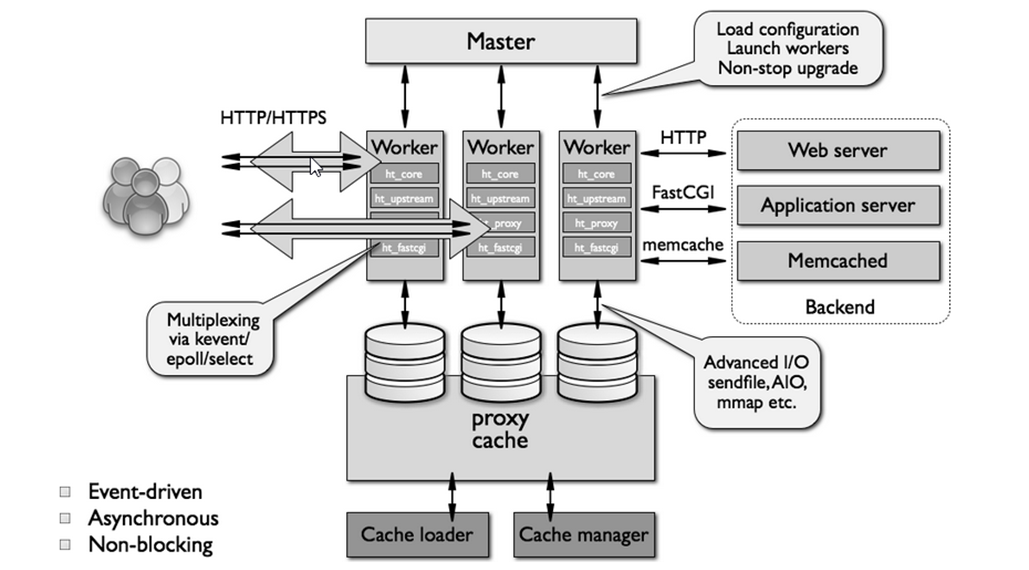
\includegraphics[scale=1]{figuras/nginx-how-it-works} 
\caption{Modelo de funcionamento do Nginx.}
\label{fig:nginx-comofunciona}
\end{figure}
O Nginx é utilizado por vários sítios de grande tráfego como Netflix, GitHub, 
Pinterest, dentre outros.\\
\section{ApacheBench}
O ApacheBench foi criado em 1996 por Adam Twiss e, posteriormente doado ao 
Apache \textit{Group}. Originalmente, a ferramenta foi desenvolvida para 
verificar o desempenho em servidores HTTP Apache, mas hoje é utilizada para 
fazer testes de desempenho em  praticamente qualquer servidor HTTP.
\section{FastCGI}
De acordo com \citeonline{fastcgi} FastCGI é uma interface para servidores 
\textit{web} rápida, aberta e segura, que resolve os problemas de desempenho 
herdados do CGI, sem introduzir \textit{overhead} e complexidade de APIs 
proprietárias.
\subsection{\textit{Common Gateway Interface}}
A interface de fato de aplicações em servidores \textit{web} é o CGI, 
implementado pela primeira vez nos servidores da NCSA. O CGI tem muitos 
benefícios:
\begin{itemize}
	\item Simplicidade: é fácil de entender;
	\item Independente de linguagem: Aplicações em CGI podem ser escritas em quase todas a linguagens;
	\item Isolamento do processo: Como os processos são executados 
	separadamente, aplicações com problema não param ou acessam o estado 
	interno do servidor \textit{web};
	\item Padrão aberto: CGI já foi implementado em praticamente todos os 
	servidores;
	\item Independência de arquitetura: O CGI não é ligado a uma arquitetura de computador em particular.
\end{itemize}
CGI tem alguns inconvenientes significantes, sendo o principal problema  o 
desempenho: como um novo processo é criado para cada requisição e descartada 
quando a requisição acaba, a eficiência é baixa.
\subsection{Servidor de API}
Em resposta ao problema de desempenho do CGI, várias empresas desenvolveram API's para os seus servidores.\\
Aplicações conectadas em um servidor de API pode ser significativamente mais 
rápido do que programas desenvolvidos em CGI. O problema da inicialização do 
CGI é melhorada, pois a aplicação é executada no processo do servidor e 
persiste pelas requisições. As API's dos servidores \textit{web} também 
oferecem funcionalidades adicionais comparadas com o CGI. O desenvolvedor pode 
criar extensões que permitem realizar controle de acesso, pegar um acesso dos 
aquivos de registro (\textit{log}) do servidor e, se conectar a outros estágios 
do processamento de uma requisição do servidor. No entanto, API's sacrificam 
todos os benefícios do GCI. São eles:
\begin{itemize}
	\item Complexidade: API's de empresas introduzem uma curva de aprendizado, 
	custos de implementação e manutenção maiores;
	\item Dependência de linguagem: as aplicações devem ser escritas na 
	linguagem de programação suportada pela API;
	\item Não há isolamento de processos: como o processo é executado dentro do 
	endereço de memória do servidor, aplicações com problemas podem corromper o 
	núcleo do servidor, comprometer a segurança e problemas no núcleo do 
	servidor podem corromper as aplicações;
	\item Proprietário: Codificar a aplicação para uma determinada API força o desenvolvedor a utilizar aquele servidor em particular;
	\item Arquiteturas de computador iguais: As aplicações devem usar a mesma 
	arquitetura do servidor \textit{web}.
\end{itemize}
\subsection{FastCGI}
A interface do FastCGI combina os melhores aspectos do CGI e das API's proprietárias. Assim como o CGI, o FastCGI executa os processos de forma separada e isolada. As vantagens do FastCGI incluem:
\begin{itemize}
	\item Desempenho: Os processos do FastCGI são persistentes, sendo 
	reutilizados para manipular várias requisições, resolvendo o problema da 
	criação de novos processos para cada requisição;
	\item Simplicidade com fácil migração do CGI: a biblioteca de aplicação do FastCGI simplifica a migração de aplicações existentes feitas usando CGI. Aplicações feitas utilizando a biblioteca de aplicações do FastCGI podem ser executadas como programa CGI;
	\item Independência de linguagem: Assim como o CGI, as aplicações FastCGI 
	podem ser escritas em qualquer linguagem;
	\item Isolamento de processos: Uma aplicação com problemas não pode 
	corromper o núcleo do servidor ou de outra aplicação.
	\item Independência de arquitetura: O FastCGI não é ligado a uma arquitetura de computador em particular. Qualquer servidor \textit{web} pode implementar a interface do FastCGI;
	\item Suporte à computação distribuída: FastCGI provê a habilidade de 
	executar aplicações remotamente, o que é útil para distribuir carga e 
	gerenciar sítios da \textit{web} externos.
\end{itemize}
\section{HTML}
De acordo com o \citeonline{w3chtml} a Web é baseada em 3 pilares:
\begin{itemize}
\item Um esquema de nomes para localização de fontes de informação na Web a URI 
(\textit{Uniform Resource Identifier});
\item Um Protocolo de acesso para acessar estas fontes, hoje o HTTP;
\item Uma linguagem de Hipertexto, para a fácil navegação entre as fontes de informação: o HTML.
\end{itemize}
\subsection{Hipertexto}
HTML é a abreviação para \textit{Hypertext Markup Language} - Linguagem de 
Marcação de Hipertexto. Em resumo, HTML é uma linguagem para publicação de 
conteúdo (texto, imagem, vídeo, áudio e etc) na \textit{web}.\\
HTML é baseado no conceito de Hipertexto. Hipertextos são conjuntos de 
elementos – ou nós – ligados por conexões. Estes elementos podem ser palavras, 
imagens, vídeos, áudio, documentos etc.. Estes elementos conectados formam uma 
grande rede de informação que não estão conectados linearmente como se fossem 
textos de um livro, onde um assunto é ligado ao outro seguidamente. A conexão 
feita em um hipertexto é algo imprevisível que permite a comunicação de dados, 
organizando conhecimentos e guardando informações relacionadas.\\
Para distribuir informação de maneira global, é necessário haver uma linguagem 
que seja entendida universalmente por diversos meios de acesso. O HTML se 
propõe a ser esta linguagem. Desenvolvido originalmente por Tim Berners-Lee o 
HTML ganhou popularidade quando o \textit{Mosaic - browser}, desenvolvido por 
Marc Andreessen na década de 1990, ganhou força. A partir de então, 
desenvolvedores e fabricantes de navegadores passaram a utilizar o HTML como 
base, compartilhando sas mesmas convenções.\\
\subsection{HTML}
Entre 1993 e 1995, o HTML ganhou as versões HTML+, HTML2.0 e HTML3.0, onde 
foram propostas diversas mudanças para enriquecer as possibilidades da 
linguagem. Contudo, até 1.995 o HTML ainda não era tratado como um padrão. 
Apenas em 1997, o grupo de trabalho W3C, responsável por manter o padrão do 
código, trabalhou na versão 3.2 da linguagem, fazendo com que ela fosse tratada 
como padrão.\\
Desde o começo o HTML foi criado para ser uma linguagem independente de 
plataformas, navegadores e outros meios de acesso. Interoperabilidade significa 
menos custo. O desenvolvedor cria apenas um código HTML e este código pode ser 
lido por diversos dispositivos ao invés de versões diferentes para cada 
dispositivo. Dessa forma, evita-se que a \textit{Web} seja desenvolvida em uma 
base proprietária, com formatos incompatíveis e de forma limitada. Por esses 
motivos o HTML foi desenvolvido para que essa barreira fosse ultrapassada, 
fazendo com que a informação publicada por meio deste código fosse acessível 
por dispositivos e outros meios com características diferentes, não importando 
o tamanho da tela, resolução, variação de cor, dentre outros. O HTML deve ser 
entendido universalmente, dando a possibilidade para a reutilização dessa 
informação de acordo com as limitações de cada meio de acesso.
\section{PHP}
PHP (acrônimo para preprocessador de hipertexto) é uma linguagem de programação 
de código aberto, interpretada, de propósito geral, de tipagem dinâmica e 
fraca, procedural, reflexiva, orientada a objetos e funcional; criada em 1.995 
por Rasmus Lerdorf. A linguagem é melhor utilizada para criação de sistemas 
baseados na \textit{web}, já que pode ser inserida diretamente em códigos 
HTML.\\
De acordo com \citeonline{phpwhatcando}, o PHP pode realizar qualquer tipo de 
atividade computacional. Tem como foco executar tarefas do lado do servidor, 
realizando qualquer tarefa que uma aplicação feita em CGI pode fazer tais como: 
coletar dados de um formulário, gerar páginas com conteúdo dinâmico ou enviar e 
recebe \textit{cookies}. Existem três áreas onde o PHP é mais utilizado:
\begin{itemize}
	\item \textit{Script} do lado do servidor: é a forma mais tradicional e o 
	principal foco do PHP;
	\item \textit{Script} de linha de comando: é uma forma de utilizar o PHP 
	sem um servidor \textit{web} ou navegador de internet. Esse forma de uso é 
	ideal para rotinas programadas executadas no sistema operacional. Pode ser 
	usada também para tarefas de processamento de texto;
	\item Aplicações para \textit{Desktop}: PHP provavelmente não é a melhor 
	linguagem para desenvolver aplicações com interface gráfica para 
	computadores de mesa, mais pode ser utilizada para criação de aplicações do 
	lado do cliente utilizando o a extensão PHP-GTK, não distribuída de forma 
	oficial pelos mantenedores da linguagem PHP.
\end{itemize}
Para fazer o PHP funcionar é preciso três coisas: Um interpretador, um servidor 
\textit{web} e um navegador de \textit{internet}. Pode ser utilizado em 
praticamente todos os sistemas operacionais e ser executado em qualquer 
servidor \textit{web} que utilize a extensão FastCGI PHP.\\
Com o PHP, o desenvolvedor não fica limitado a somente gerar páginas HTML, 
incluindo as habilidades de entregar imagens e arquivos em geral, geração de 
páginas em XHTML e qualquer outro arquivo XML e servindo como \textit{cache} no 
servidor para o conteúdo gerado dinamicamente.\\
Uma das funcionalidades mais importantes do PHP é o suporte a uma grande 
variedade de bancos de dados. Desenvolver páginas que utilizam base de dados é 
simples, desde que se use uma extensão para base de dados presente na 
linguagem, uma camada de abstração, como por exemplo o PDO, ou conectar a 
qualquer base de dados que suporte o padrão ODBC.\\
O PHP tem ferramentas de processamento de texto úteis, incluindo analisador de 
expressões regulares compatível com a linguagem de programação Perl, além de 
várias outras extensões e ferramentas para analisar e acessar documentos no 
formato XML.
\subsection{PHP-FPM}
O PHP-FPM (\textit{(FastCGI Process Manager}) é uma implementação alternativa do PHP FastCGI com algumas funcionalidades úteis, principalmente, para sítios com grande acesso. Essas funcionalidade incluem:
\begin{itemize}
	\item Gerenciamento avançado de processos;
	\item Habilidade para iniciar processos com diferentes usuários, grupos e ambientes, escutando portas diferentes e usando diferentes arquivos de configuração;
	\item Registro (\textit{log}) de atividades nas saídas padrão de texto 
	(stdout) e de erros (stderr) do sistema operacional;
	\item Reinicialização emergencial em caso de destruição acidental da memória cache;
\end{itemize}
\section{PostgreSQL}
De acordo com \citeonline{postgresql} PostgreSQL é um sistema gerenciador de banco de dados objeto-relacional que tem sido desenvolvido de várias formas desde 1.977. Começou como um projeto chamado Ingres na \textit{University of California} em Berkeley, Estados Unidos. O Ingres foi, posteriormente, desenvolvido comercialmente pela empresa Relational Technologies.\\
Em 1.986 uma outra equipe chefiada por Michael Stonebraker continuou o desenvolvimento do código do Ingres para criar um sistema de banco de dados usando o paradigma objeto-relacional chamado Postgres. Em 1.996, o Postgres foi renomeado para PostgreSQL.\\
O PostgreSQL é considerado por muitos o melhor SGBD de código aberto do mundo, 
provendo várias funcionalidades que, normalmente, são vistas somente em 
produtos comerciais desenvolvidos para grande empresas.\\
\section{Miolo \textit{framework}}
O Miolo é um \textit{framework} para criação de sistemas de informação 
acessíveis via \textit{web} escrito em PHP. O Miolo utiliza \textit{scripts} 
javascript e conceitos de programação orientada a objetos, gerando páginas HTML 
e arquivos PDF. Com um projeto modular, baseado em componentes, e uma 
arquitetura em camadas, o Miolo atua como ``\textit{kernel}'' de todos os 
sistemas criados. Favorecendo a reutilização, os vários sistemas podem ser 
facilmente integrados, funcionando como módulos de um sistema mais complexo. 
Além de proporcionar as funcionalidades para o desenvolvimento de sistemas, o 
Miolo também define uma metodologia de codificação para que os resultados 
esperados sejam obtidos de forma simples e rápida.\\
Os sistemas desenvolvidos com o Miolo seguem algumas regras básicas que devem 
ser conhecidas, como as definições de classes/\textit{forms}/\textit{handlers} 
dos módulos, definição dos arquivos de configuração (localização dos programas, 
componentes, bancos de dados, temas, etc.), o ciclo de vida de execução de uma 
requisição do cliente, além das principais classes, métodos e controles. 
Algumas das principais funções implementadas pelo framework são:
\begin{itemize}
	\item Controles de interface com o usuário, escritos em PHP e renderizados 
	em HTML;
	\item Autenticação de usuários;
	\item Controle de permissão de acesso;
	\item Camada de abstração para acesso a bancos de dados;
	\item Camada de persistência transparente de objetos;
	\item Gerenciamento de sessões e estado;
	\item Validação de entrada em formulários;
	\item Customização de \textit{layout} e temas usando CSS;
	\item Geração de arquivos em PDF;
\end{itemize}
